%!TEX root = ../template.tex
%%%%%%%%%%%%%%%%%%%%%%%%%%%%%%%%%%%%%%%%%%%%%%%%%%%%%%%%%%%%%%%%%%%%
%% chapter2.tex
%% NOVA thesis document file
%%
%% Chapter with the template manual
%%%%%%%%%%%%%%%%%%%%%%%%%%%%%%%%%%%%%%%%%%%%%%%%%%%%%%%%%%%%%%%%%%%%

\typeout{NT FILE chapter2.tex}%

\chapter{Literature Review}
\label{cha:literature_review}

\textit{This section provides an overview of the relevant research related to the topic of the project. Starting with highlighting the importance of understanding the mechanism of action for enhanced drug discovery. The following sections detail two key components for MoA elucidation through computational analysis. First, the transcriptomics data and networks serve as a foundation for the analysis. Next, it outlines the computational methods used to apply various scoring algorithms: topology-, similarity-, and enrichment-based algorithms. Together, these components form the basis of our systematic evaluation of tools for elucidating compound MoA. Finally, an overview of the best practices to perform a benchmarking study is provided.}

\section{Drug discovery: the importance of the compound’s mechanism of action} % (fold)
\label{sec:drug_discovery:_the_importance_of_the_compound’s_mechanism_of_action}

\cite{viper}

The development of new drugs is a highly complex process in the R\&D field. The high prevalence of complex diseases today, which collectively account for 70\% of all deaths in Europe and affect approximately 25\% of the population, is one of the challenges faced by this industry [12]. In addition, statistics show that de novo drug discovery has become an extensive and costly process, taking around 13 years and with a cost as high as \$2 billion to develop a new drug, with clinical trials lasting an average of approximately 95 months and non-clinical phases lasting 31 months [13-15]. These challenges have led to fewer drug approvals by regulatory bodies, resulting in a significant gap between therapeutic demand and available treatments. Hence, as the current treatments become less effective, there is a strong interest in finding alternatives to optimize critical steps in the drug development pipeline and developing more advanced therapeutic methods [16]. Efforts to address these challenges are evident in the growing number of studies, both in industry and academia. However, this is still not enough to meet the growing need for new drugs. 
Drug repositioning (DR) has emerged as a promising cost-effective strategy to tackle the constraints faced by traditional DD by reducing the initial cost to 1/3 and the duration to 3-9 years. It continues to gain increasing attention, as nearly 30\% of the drugs and vaccines approved by the FDA are derived from this method [17, 18]. The fundamental goal of DR is to broaden the scope of the known, safe, and previously approved drugs for other diseases. This is a particularly interesting method for both perspectives of drugs and diseases. By offering ways not only to investigate treatments that have been put on hold because of failed clinical trials [19], but also for diseases where no effective treatment is known, especially rare diseases, which big pharma is not particularly interested in investing in when using traditional blinded methods, given the low financial return. Many studies have demonstrated the success of establishing new drug-disease relationships [20]. A well-known example is Sildenafil; initially identified in the 1980s as a candidate to treat angina pectoris, it was approved by the Food and Drug Administration (FDA) in 1998 to treat erectile dysfunction and later in 2005 to treat pulmonary arterial hypertension [17, 18, 21]. Another classic example is Thalidomide, originally used for sedation and morning sickness, and afterward repurposed for multiple myeloma, leprosy [17, 18], and to minimize the hippocampal neuronal loss [22]. Moreover, the low success approval rate (5\%) of cancer treatments that enter phase I clinical trials led to increased attention in DR for oncology, resulting in several promising findings [18, 23]. Noteworthy cases include the schizophrenia drug Spiperone, which has been studied for its ability to induce apoptosis in colorectal cancer (CRC) cells [24], and Raloxifene, indicated for osteoporosis, which proved to be effective in reducing invasive breast cancer risk in postmenopausal women [18, 25].
Understanding how cellular signaling (Figure 1) is modulated upon disturbance within an organism is essential for identifying potential drug targets and finding new indications for an existing drug or a disease that a known drug could treat. When a drug enters a biological system, it typically interacts directly or indirectly with cellular targets and therefore regulates the activity of signaling networks and pathways, a process known as the mechanism of action (MoA) [26, 27]. These interactions impact the course of drug R\&D, from initial investigation to clinical trials, and deep comprehension of these mechanisms can help uncover important biomarkers, anticipate early adverse effects, and even synergistic effects resulting from drug combinations. Nevertheless, FDA approval can be obtained without knowing the drug’s MoA if the drug exhibits safety and efficacy [28, 29]. Yet, not knowing the mechanisms of the compounds can be extremely disadvantageous, as demonstrated with Dimebon, which could have taken a different course if its MoA had been initially characterized. Originally developed as an antihistamine, it later entered clinical trials, with the MoA still unknown, as a treatment for Alzheimer’s but failed in the third phase of the study for not affecting cognition, since it was the activation of histamine and serotonin receptors that caused the initial observed cognitive efficacy and not the stabilization of mitochondria as first hypothesized [28, 30]. 
Although we refer to the target(s) of a compound as a direct interaction, this is not the case. Subsequently, there is a series of interactions that modulate the different levels of biological data, and what is “detected” at a given moment does not always linearly reflect what happened previously. Indeed, the basic definition of MoA is just the tip of the iceberg, given that the chain of reactions triggered involves various molecules and forms the cell signaling cascade. This cascade is characterized by the pathways through which the signal moves within the cell and which lead to certain cellular responses. These pathways can also interact with each other through crosstalk [31], forming a network, which, although interconnected, are distinct concepts. The impact of a certain compound in the complex cell signaling cascade can be defined and observed on a system level by different multi-omics layers, such as genomics, transcriptomics, proteomics, metabolomics, and even phenomics, each offering an alternative perspective on the compound’s bioactivity. However, finding experimentally which targets, signaling proteins, and biological pathways (MoA) are being modulated by an uncharacterized compound can be a huge barrier in the process of drug discovery. Owing to the advantages of clearly describing the MOA more quickly and affordably, along with the increasing availability of high-throughput data, in silico methods have become an attractive option. These methods act as a pre-filtering process, helping to identify and produce mechanistic hypotheses for further experimental validation [28]. Many accessible computational resources integrate “omics” data with prior knowledge graphs, such as gene regulatory networks, to enhance and pinpoint the drug's potential cellular targets. However, choosing the most suitable data and computational tool to employ in each situation is not always simple, so it is important to determine exactly the scientific question that needs to be addressed. By doing this, researchers may choose the most appropriate data type and bioinformatics tools to efficiently study the compound's mechanism of action.

\section{Transcriptomics data}
\label{sec:Transcriptomics_data}

Transcriptomics data provide a comprehensive view of gene expression level changes in response to a compound. Following the compound’s perturbation, this data will reflect the differential mRNA expression by capturing modulated signaling and transcription factor activity changes triggered by the perturbagen, therefore, it is a type of data that plays a crucial role in understanding a compound's MoA. After a cellular disturbance, changes in gene expression levels give rise to a perturbed gene expression signature [32]. In 2000, a reference database was built from a compilation of Saccharomyces cerevisiae gene expression signatures derived from pharmacological and genetic perturbations, and the same authors even projected that to generate a wider collection of reference signatures, less expensive gene expression experiments would be required [33-35]. Since then, and with the growing interest in drug discovery optimization, several databases have emerged to aggregate and publicly provide perturbagen transcriptomic signatures. These databases make it possible to extract information on how gene expression is modified by certain manipulations and treatments (~\ref{tab:transcriptomics_resources}). 
DrugMatrix was the first larger molecular toxicology database, created in 2006 by Iconix Pharmaceuticals, later acquired by the National Institute of Environmental Health Sciences (NIEHS), and has been publicly available since 2011 [33, 36, 37], comprises the gene expression response obtained through microarray to more than 600 perturbagens in rat tissues.  Additionally, it provides information on chemical treatments related to histopathology, hematology, and clinical chemistry, enabling the investigation of certain types of toxicity [38]. However, studies in vivo limit the number of disturbances that can be studied, entail high costs that make it impractical to generate data on a large scale, as well as all the associated ethical implications [9]. In addition, transcriptional changes are usually specific to each cell, so a precise analysis of transcriptomic changes before and after perturbations should be carried out, considering the cell type, which requires even more resources [39].
Connectivity mapping (CMap) is a resource that emerged from an attempt to address the lack of a systematic way to establish connections between the MoA of chemical compounds, diseases, and biological processes through pattern matching between signatures derived from perturbations applied to different cell lines. The first version of CMap (CMap 1.0) generated 453 signatures derived from 164 distinct perturbations of small molecules applied at two time points under certain concentrations to four human cell lines (MCF7, PC3, HL60, and SKMEL5) [9]. Although the goal could be achieved using signatures from various -omics layers, to capture cellular response at different levels, this resource focused only on mRNA expression data through DNA microarrays. While the concept behind this database has become extensively utilized, the data generated by this pilot project was too small for the potential application of this tool. The perturbations were few and undiversified in terms of perturbations and cell lines. The recent advances in high-throughput technology, allowed large data acquisition, as is the case with the L1000 assay. The Library of Integrated Network-Based Cellular Signatures (LINCS) program extended the CMap to a second version (CMap 2.0 or LINCS L1000) that measured the expression of 978 “landmark” genes, key representatives of various biological processes, in cells treated with different perturbagens [40]. Using the Luminex L1000 platform, these landmark genes are directly measured, and computational methods and in silico imputation then infer the expression of 11350 additional genes, resulting in a wider reconstruction of the genome profile [47]. In a preliminary phase, LINCS released over 6000 signatures from around 1300 small compounds, many of which were FDA-approved [33], and today it includes more than one million gene expression profiles from over 20000 chemical and genetic perturbagens, tested at multiple time points and doses across various human cell lines. Currently, the dataset is more than a thousand times larger than the CMap pilot dataset. The perturbagens include small-molecule compounds and genetic treatments, such as gene knockdowns using short hairpin RNA (shRNA) and/or CRISPR and induced over-expression (OE). LINCS L1000 provides data in five levels. Levels 1 to 4 contain data at different pre-processing stages, and Level 5 contains the final signatures, where replicates, usually three per treatment, are combined into a single differential expression vector. This level is recommended for most downstream analyses [40]. The extension of data by LINCS L1000 has broadened the association between changes in gene expression caused by certain disorders, enhancing the repositioning of drugs and contributing to the generation of testable hypotheses about the MoA of less characterized compounds. However, the additional genes are imputed and not measured directly, which can lead to some inaccuracy. In addition, the inherent complexity of cellular responses must be considered, since gene expression snapshots may not fully capture the dynamic nature of biological processes and do not always correlate perfectly with protein expression due to post-translational modifications [27]. Despite these limitations, several computational methods have been developed to apply these data for leveraging the drug discovery process. However, the interpretation of the results must be careful to consider the static and imputed nature of the data. These methods will be described later in this chapter. 
The Cancer Drug-induced Gene Expression Signature Database (CDS-DB) [41] is an interactive, user-friendly resource, released in September 2023, aiming to provide data on how cancer therapies affect gene expression in patient samples. It compiles gene expression profiles from 78 patient-derived paired pre- and post-treatment datasets, from GEO and ArrayExpress databases, with manually curated clinical information. These source datasets have been organized into 219 CDS-DB datasets, composed of the gene expression levels from paired pre- and post-treatment patient samples, with the same factors (therapeutic regimen, administration dosage, cancer subtype, sampling location, time, and drug response status). From those, datasets with at least two patients have been used to generate differential expression analyses, resulting in 181 dataset-level gene perturbation signatures. In addition, 2012 patient-level gene perturbation signatures have been derived by comparing pre- and post-treatment profiles from individual patients (e.g., baseline vs. 14-day; baseline vs. three months). All transcriptomic data in CDS-DB were uniformly re-processed from raw files (microarray or RNA-seq), the metadata was manually curated, and the terminologies for drugs, cancers, and genes were harmonized. This database is an important resource for MoA elucidation studies by providing well-curated gene expression data for various cancer types and treatments, and by distinguishing between dataset-level signatures (group-level differential expression) and patient-level signatures (individual patient responses) [41]. Nonetheless, CDS-DB only provides data from cancer patient samples, and in LINCS, the cancer cell lines represent nearly all the gene expression profiles, so they are not ideal for addressing the challenges related to transcriptional responses in non-cancer cells [39].
ChemPert [39], emerged as a manually curated resource that maps the relationships between chemical perturbations, their protein targets, and downstream transcriptional signatures in non-cancer cells. It provides a user-friendly interface that includes two sections: the database and a web analysis tool. The database has three main components: (1) Direct signaling protein targets of chemical perturbagens, curated from Drug Repurposing Hub, DrugBank, and STITCH v5.0; (2) Initial gene expression profiles of non-cancer cells before exposure, extracted from GEO, ArrayExpress, and LINCS L1000 (Level 3 data); (3) Transcriptional responses after perturbation, categorized as upregulated or downregulated. The ChemPert database encompasses over 82000 transcriptional signatures from the exposure to 2566 chemical compounds across 167 different non-cancer cell types, lines, and tissues. It includes target data for 57818 chemical compounds, capturing activation, inhibition, or unknown effects. Additionally, ChemPert also offers two built-in analysis tools: (1) Given a perturbagen and the initial gene expression profile, the users can predict how transcription factors will respond; (2) Given a specific transcriptional response the users can identify the potential perturbagens based on that input data. 
Bulk transcriptomic databases average gene expression across cells, potentially masking important heterogeneity responses between different cells to perturbations, such as the existence of cell subpopulations that can survive chemotherapy [42]. To capture these variations, single-cell perturbation sequencing methods have emerged. Techniques like Sci-Plex (for chemical perturbations) and Perturb-seq (for genetic perturbations) leverage mass screening technologies in combination with single-cell resolution to provide a more detailed view of cellular responses [43]. Although traditional single-cell RNA sequencing (scRNA-seq) is essential for analyzing such heterogeneity, its high cost per sample remains a barrier. Sci-Plex [42] was introduced to overcome this limitation by combining two techniques: nuclear hashing and combinatorial indexing-based RNA sequencing (sci-RNA-seq) to assess the global transcriptional responses to chemical perturbations at single-cell resolution [44, 45]. Nuclear Hashing labels cell nuclei with unique DNA barcodes before pooling, allowing multiple treatment conditions to be multiplexed in one experiment. Sci-RNA-seq uses successive rounds of combinatorial indexing to uniquely tag transcripts from individual cells, enabling high-throughput scRNA-seq at a much lower cost.

\begin{newpdflayout}{210mm}{297mm}%{420mm}

% \bgroup
% %\rowcolors{1}{}{GhostWhite}
% \begin{xltabular}{\textwidth}{Xccccc}
% \caption{List of resources that provide transcriptomics data-driven from perturbagen.}
% \label{tab:transcriptomics_resources}\\
% \toprule
% %\rowcolor{Gainsboro}%
% \textbf{Database}   & \textbf{Description} & \textbf{Reference} \\
% \midrule
% ArrayExpress        & ArrayExpress is a curated repository of functional genomics experiments (non-toxicity specific), including microarray and HTS data from various perturbation studies. Established in 2003, it maintains high-quality standards through curation, offering structured metadata and accessioned datasets for diverse biological conditions, including compound treatments and diseases. It provides access to the data from other resources, such as DrugMatrix [46] and Open TG-GATES [38].            & Compound            \\
% CDS-DB              & Cancer Drug-induced gene expression Signature DataBase (cdsdb) is a patient-derived cancer drug response database that compiles pre- and post-treatment microarray and RNA-seq data. It provides data for a better understanding of the treatment effects, drug response, and resistance mechanisms. It includes curated metadata from GEO [48] and ArrayExpress [47] sources and supports data browsing, searching, and single signature analysis.             & CRISPR KO           \\
% LINCS OE            & Chemical Effects in Biological Systems is a publicly accessible repository for toxicogenomic data (cebs), established in 2008. It integrates multiple types of experimental data, including detailed study designs and timelines, clinical chemistry profiles, histopathological findings, as well as microarray and proteomics data, collected from studies examining both chemical exposures and genetic alterations [49].             & ?                   \\
% LINCS shRNA a375           & ChemPert (chempert) is particularly useful for comprehending the molecular impacts of chemicals in non-cancer cellular contexts. It provides 82270 manually curated transcriptional signatures derived from 167 non-cancer cell types in response to 2566 perturbagens, such as small molecules, drugs, cytokines, and growth factors. It also includes the protein targets for 57818 chemical compounds, and the respective effect (activation, inhibition, or unknown).             & ?                   \\
% ChemPert                   & Chemical            & 2                   \\
% CREEDs                     & Chemical            & 2                   \\
% CDS-DB                     & Chemical            & 1                   \\
% PertOrg                    & Genetic             & 1                   \\
% GWPS                       & Genetic             & 2                   \\
% Sci-Plex                   & Chemical            & 3                   \\
% %\midrule
% %\rowcolor{Gainsboro}%
% \bottomrule
% \end{xltabular}
% \egroup

\begin{center}  
\begin{tabular}{ | l | l | l | p{5cm} |} % you can change the dimension according to the spacing requirements  
\hline  
Database    & Description      & Reference \\ \hline  
Orange      & Fruit     & It is fruit, which is full of nutrients and low in calories. They can promote clear, healthy skin and also lowers the risk for many diseases. It reduces cholesterol and also helps in building a healthy immune system.\\ \hline  
Cauliflower & vegetable & It is the vegetable, which is high in fiber and B-Vitamins. It also provides antioxidants, which help in fighting or protect against cancer. It enhances digestion and has many other nutrients.\\ \hline  
\end{tabular}  
\end{center}

\end{newpdflayout}


Sci-Plex was applied to three well-characterized human cancer cell lines, A549 (lung adenocarcinoma), K562 (chronic myelogenous leukemia), and MCF7 (mammary adenocarcinoma), exposed to 188 different compounds at four doses [42]. The integration of the two techniques allowed for profiling thousands of single-cell transcriptomes across nearly 5000 independent samples simultaneously in one experiment. Genome-wide Perturb-seq (GWPS) is a large-scale database that maps how genetic changes affect cell behavior by using a single-cell genetic perturbation sequencing (Perturb-seq), a CRISPR interference (CRISPRi) screening technique combined with single-cell RNA sequencing [54]  [54]. In this approach, every expressed gene was silenced at the genome-scale to capture detailed transcriptional responses. This massive dataset allowed them to assign functions to previously uncharacterized genes and to identify new regulators involved in key cellular processes such as ribosome biogenesis, transcription, and mitochondrial respiration [54]. Additionally, the rich single-cell data enabled a deep exploration of complex phenomena, including RNA processing, differentiation, and stress-specific regulation, particularly in the context of aneuploidy. Comprehensive analysis of cellular changes in response to perturbations has been made possible by high-dimensional transcriptional profiling of cells. High-resolution single-cell expression data holds great promise for detecting cell-level transcriptional alterations across experimental conditions, because many disturbances only impact a portion of a certain cell type, with most of the cells remaining unaffected. 
Gene Expression Omnibus (GEO) is a public repository managed by the National Center for Biotechnology Information (NCBI) that archives microarray and next-generation sequencing data from various organisms, cell lines, etc [48]. The vast array of high-throughput experimental data stored in this resource frequently serves as the foundation for more specialized databases, making it difficult to mention other databases without mentioning GEO. Additionally, querying GEO often requires manual sample identification that has been subjected to disturbance and the control samples, since this database does not have an obligation to publish the metadata accurately [33]. When the data is user-submitted and publicly available, sometimes it ends up being unfeasible to use due to the lack of associated metadata. Other databases use the data originally from GEO, after curation and ensuring that all the associated metadata are provided, to overcome the lack of this in-depth information that often exists. The CRowd Extracted Expression of Differential Signatures (CREEDS) is a gene expression signature database that resulted from a crowdsourcing project to improve the annotation and reanalysis of data from the GEO [51]. By engaging over 70 participants, several datasets with single-gene, drug, and disease perturbation signatures were manually curated and validated for accuracy. These signatures were then used as a training set for machine learning models, allowing the collection to be scaled up with an automated search. CREEDS tackles the key challenge of metadata inconsistencies and lack of standardized annotation by using both manual curation and computational methods such as the characteristic direction algorithm to prioritize the DEGs [51]. The platform enables the download of human-validated gene expression signatures, with reduced error in control and perturbation selection, unlike signatures available from fully automated signature extraction tools.
PertOrg 1.0 [56] is another database built on extracted data from GEO [48] and ArrayExpress [47] databases to construct a comprehensive tool to analyze and download curated gene expression and phenotypic data from genetically modified organisms. This extensive database catalogs induced in vivo genetic perturbations across 8 diverse model organisms including mammals (mouse and rat), non-mammalian vertebrates (zebrafish), invertebrates (nematode worm and fruit fly), microorganisms (bacteria and yeast), and plant (thale cress). The database includes various types of genetic modifications, such as gene knockout (complete removal or inactivation of a specific gene), gene knockdown (partial suppression of gene expression using RNAi or similar techniques), gene overexpression (increased expression of a target gene through vector-based methods), and mutations and other genetic modifications (specific point mutations, insertions, or deletions introduced to study gene function and disease models). PertOrg has identified over 8.6 million DEGs associated with genetic modifications, derived from microarray, RNA-seq, and scRNA-seq. The database has two main built-in analytical tools, the differential gene overlapping analysis which investigates perturbation datasets significantly enriched in the user-given gene set using a hypergeometric test, and dataset enrichment analysis which identifies perturbation datasets where the user-given gene set is over-represented [56]. The huge collection of curated non-human data and all the functionalities offered make this a valuable resource, bridging the gap between genetic disorders and their phenotypic outcomes.
Perturbation signatures can provide valuable information about the key targets and pathways involved in the compound’s effect through the gene expression changes. However, extracting downstream information is not an easy task itself, so integrating transcriptomics data with prior knowledge networks allows the mapping of gene regulatory networks and a better understanding of the complex interactions and regulatory mechanisms behind the snapshot provided by a perturbation signature.


\section{Prior knowledge Network} % (fold)
\label{sec:Prior_knowledge_Network}

Understanding the physical molecular interactions within a biological system is crucial for contextualizing experimental data. Computational methods for elucidating the mechanisms of action allow the integration of omics data with prior knowledge of the interactions between biological entities [28].  These interactions can be represented with more or less complexity and can be included in the analysis as supplementary data sources. A prior knowledge network (PKN) is a collection of interactions where nodes represent molecular entities (such as proteins, genes, or metabolites) and edges illustrate their relationships. Understanding causal graphs is key to modeling and interpreting these networks, as they depict cause-and-effect relationships. In such graphs, nodes represent variables, while directed edges represent causal influences, indicating that a change in one variable affects another [60]. Furthermore, edges can be signed, indicating whether a causal node employs a positive or negative effect on the second variable, and weighted, to show the connection strength [60]. In causal graphs that model biological networks, multi-edge connections are common, with two or more edges linked to the same node. 
Networks can be classified based on interaction types and node characteristics. Protein-protein interaction (PPI) networks show direct interactions between proteins. Gene Regulatory Networks (GRN) Figure \ref{fig:regulons} illustrate how transcription factors influence gene expression [1]. Signal transduction networks describe how cells process external signals. Metabolic networks display relationships between enzymes and metabolites. Furthermore, networks are not always composed of molecular entities, as is the case with the disease network model, which links diseases using genes and mutations as connections. These networks fit experimental data to predictions from causal graphs describing the system. The choice of the PKN should match the data type. For instance, for transcriptomic data, integrating a Protein-Gene Regulatory Network (PGN) may be beneficial, while for metabolomic data, metabolic networks are more suitable. Researchers have made significant efforts to construct regulatory networks. A primordial example was the functional characterization of yeast genes through PPI analysis. This study aimed to show the guilt-by-association principle, by inferring an unknown protein's function by looking at its interactions with nearby entities [60, 61]. The guilt-by-association principle is a foundational concept in biological networks. It suggests that genes with similar functions often interact with the same proteins or have similar expression patterns [62]. This principle also applies to drugs that cause similar transcriptional responses and may have comparable mechanisms of action (MoA) [18].
Biological interactions can be described with different levels of complexity. A network is an intricate representation of the global interactome, linking all entities in the system. These interactions are primarily established in published experimental research and can vary in the amount of associated information. Based on supporting studies, each interaction may include details about direction, signal, and confidence level. This helps filter data, creating a network with more reliable relationships. Still, networks can be noisy and incomplete, with high rates of false positives and negatives and a tendency for well-researched entities to become overrepresented [28, 63, 64]. In contrast, a pathway is a simpler version of a network. It illustrates a series of molecular interactions that begin with one entity and follow a specific signaling cascade. This arrangement helps classify entities by their common biological roles. Yet, pathways often miss crosstalk between other pathways and provide a static view of a dynamic process [28]. The entities’ overrepresentation issue also applies to pathways. Another way to show interactions is, for example, through regulons. Regulons are groups of co-regulated genes controlled by a common transcription factor and are usually represented as GRN (Figure 2).  The choice of network type must always be appropriate to the scientific question and the type of data with which the network is used. The interactions between biological entities and the complexity of these interactions should be considered. For example, if pathways are used instead of a full network, they might miss some interactions and changes over time. If the study targets a specific cell type or tissue, it's important to use tissue-specific networks. Databases like TissueNet [65] can provide molecular interactions specific to a particular cellular context. The use of large-scale causal graphs for gene expression data interpretation was first introduced by Pollard et al. [64, 66]. This study aimed to infer the molecular causes of the changes in oxidative phosphorylation gene expression in skeletal muscle from type 2 diabetes (DM2) patients. For this purpose, the gene expression data were integrated with a large-scale model created from over 210,000 molecular relationships based on the DM2 literature. Computer-aided causal reasoning on these complementary data identified that the observed changes are linked to decreased glucose transport, impaired insulin signaling, and increased risk of post-transplant diabetes [66]. Given the good results obtained from supplementing the studies with PKN, the identification of interactions began to receive more attention. The development of high-throughput screening techniques such as yeast two-hybrid screening and DNA microarray [67] allowed the detection of PPI. Those interactions began to be deposited in databases that provide molecular interaction data. Nowadays, there are several public and commercial network and pathway resources. Table 2 summarizes some of the main resources of biological pathways and networks. Two resources, public and commercial, that provide composite networks are OmniPath and MetaBase™, respectively. OmniPath [68] is a freely available resource of prior knowledge in molecular biology. It combines data from over 100 resources and builds five integrated databases with different types of data: Interactions (several molecular interactions organized into sub-networks), Post-Translational Modifications (enzyme-substrate reactions), Complexes (35,000+ protein complexes), Annotations (proteins and complexes annotations, such as the function, localization, tissue, etc.) and Intercell (inter-cellular signaling roles, such as, if a protein is a ligand, a receptor, an extracellular matrix component,  etc.) [68]. The interactions database is a composite signaling network that offers several manually curated subnetworks, encompassing a total of 282,504 unique interactions. Each subnetwork has different types of interactions, including post-translational interactions, transcriptional interactions, post-transcriptional interactions, and other interactions involving small molecules. The number of interactions per subnetwork is described in Figure 3. One of the GRNS that is provided by this database is the CollecTRI-derived regulons [1] Figure \ref{fig:regulons}. This collection contains high-confidence signed transcription factor (TF) - target gene interactions. These interactions were compiled from 12 resources, including information inferred from text mining, manual curations, and several publicly available databases.

\begin{figure}[htbp]
    \centering
    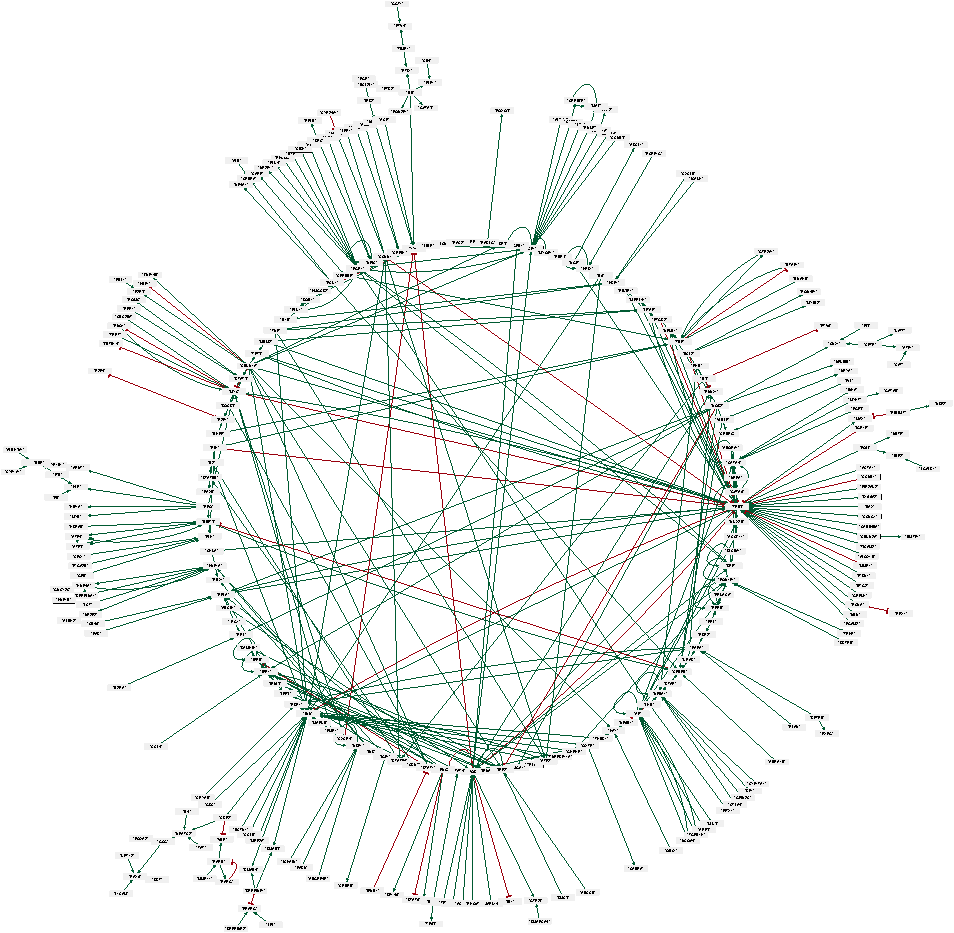
\includegraphics[height=4in]{regulons}
    \caption{Gene regulatory network based on regulon representation of human transcriptional interactions. CollecTRI-derived regulons were extracted from the decoupleR (v. 2.12.0) package, which provided 43,178 interactions. CollecTRI collection [1] is a comprehensive, curated resource of transcription factors (TFs) and their target genes, expanding on DoRothEA. This figure illustrates a subset of those 1,000 interactions, with edge color indicating the mode of regulation (green for activation and red for repression) using RCy3 (v. 2.26.0) R package.}
    \label{fig:regulons}
\end{figure}

MetaBase™ [69] is a proprietary, commercial database from Clarivate that offers one of the most comprehensive, manually curated systems biology datasets available. It contains over 4.2 million molecular interactions, including protein-protein, protein-RNA, compound-protein, compound-compound interactions, and transport reactions, with details on directionality, mechanisms, and effects. In addition, MetaBase provides more than 1,500 pathway maps that cover regulatory, disease, metabolic, and toxicity characteristics, alongside over 10,000 disease-related networks and 1,000+ validated networks. Each interaction is assigned a trust score that reflects its reliability, helping users distinguish well-established interactions from those obtained via high-throughput screening. MetaBase is accessible through SQL queries or via the metabaseR package in R, which simplifies visualization, functional analysis, and network manipulation. Furthermore, the CBDD R package offers 73 advanced algorithm implementations for analyzing and extracting insights from networks.
Integrating biological knowledge with experimental data is key to understanding how cellular regulation impacts gene expression.  Known interaction networks are usually used to predict the results of regulatory events, but they can also be used in the opposite direction, to find upstream regulators that cause expression changes [64]. Computational tools play a crucial role here. They combine high-throughput omics data with established cellular interactions, like protein-protein interactions and signaling pathways, to give a broader context. While network data show the complete interactome of molecular interactions, pathway data arrange these interactions into cascades. Each of these data sources forms prior knowledge. When combined with experimental results helps to create mechanistic hypotheses about, for instance, how a perturbation works in a system. This integration of experimental and interaction data sets the stage for some of the computational methods covered in the next chapter. These methods aim to uncover the mechanisms that cause the observed transcriptomic changes.

\section{Computational methods for MoA inference} % (fold)
\label{sec:Computational_methods_for_MoA_inference}

Due to technological advances, large-scale transcriptomics datasets can now be generated affordably across many perturbations. However, extracting biological insights from this complex data can be complicated. Thus, using computational tools has become essential for analyzing the massive amounts of data available. These methods include in silico experiments that combine experimental data with prior knowledge. They fall into three main categories: topology-based, similarity, and enrichment methods [14, 84]. Choosing the appropriate tool depends on several factors, including the type of input data, runtime, computational complexity, and the specific scientific questions being addressed, along with the inherent strengths and limitations of each method [28]. For example, in Hill et al.'s study, [60] three types of topology-based algorithms were employed. Node prioritization algorithms rank the nodes in the network based on connectivity or distance from start nodes, causal regulator algorithms infer and rank upstream nodes in the network by their connectivity or distance from start nodes, and subnetwork identification algorithms extract regions of the input network that are enriched for perturbed nodes. These approaches help generate mechanistic hypotheses about the cellular targets and pathways affected by a perturbagen more accurately and easily [85]. 

\subsection{Similarity-based methods for comparative analysis} % (fold)
\label{sub:Similarity-based_methods}

\subsection{Enrichment-based tools for downstream analysis for downstream analysis} % (fold)
\label{sub:Enrichment-based_tools}

\subsection{Topology-based methods for upstream analysis} % (fold)
\label{sub:Topology-based_methods}



\section{Benchmarking of computational methods for MoA inference} % (fold)
\label{sec:benchmarking_of_computational_methods_for_MoA_inference}

The use of computational methods to elucidate mechanisms of action is becoming increasingly indispensable for integrating and interpreting the multitude of available data. Given the plethora of existing computational tools, choosing the appropriate data and methods to answer specific scientific questions can be challenging. When a new tool is developed and published, it is usually compared with popular existing methods. For those with less experience, distinguishing the benefits of a novel tool from others that may be equally advantageous but better suited for different applications or data types can be difficult. 
A comprehensive benchmarking study of the tools is crucial for evaluating available methods in a standardized way, providing sufficient information to accurately choose the best tools and data for a given study [88]. A key component of a benchmarking study is the use of gold-standard datasets, against which the results obtained from a method are compared. By comparing these results with the ground truth, it is possible to evaluate performance metrics and statistical analyses, consistently distinguishing different computational algorithms based on their behavior with certain types of data. It is widely acknowledged that evaluating the vast available methods is important for obtaining more accurate results. Therefore, following certain good practices when conducting a benchmarking study is essential. These studies can be carried out by the authors who implemented the tool, independent groups, or as organized challenges, such as those organized by the Dialogue on Reverse Engineering Assessment and Methods (DREAM) Consortium [89]. When the authors do the evaluation, the aim is usually to demonstrate the advantages and performance improvements over other techniques. In other contexts, it is extremely important to define the scope and purpose of the benchmark. The selection of the methods should reflect the relevance of the study’s objective and include publicly available implementations to ensure accessibility. Parameter optimization can significantly affect a tool's behavior, including runtime, yet finding the optimal values is not always straightforward. Thus, balancing default settings with computational efficiency is important. Regarding datasets, in the context of studying the compound’s mechanism of action, it is crucial to include diverse data sources and generation methods to ensure representativeness and a credible assessment of performance. For instance, transcriptomic data, if making sense in the scope, should ideally include both bulk RNA-seq and single-cell RNA-seq data to broaden the options and use two widely used types of data. Since there are no perfect, fully curated datasets, it is necessary to ensure quality to avoid biasing the results and performance of the tools [89]. The same applies to the gold standard datasets, which serve as the ground truth and are fundamental for statistical analysis and assessing metrics, defining the essence of a benchmarking study.
Some benchmarking studies arise from an effort to contextualize gene expression data with several computational algorithms. Hosseini-Gerami et al. [27] evaluated the performance of different causal reasoning algorithms to recover direct compound targets of small molecules and associated signaling pathways using gene expression data. The study compared four causal reasoning algorithms against networks from two different sources and transcriptomics data from one database. Hill et al. [60] conducted a study that provided a more comprehensive framework by analyzing a diverse range of algorithms, networks, and datasets to assess how well network-based algorithms prioritize and connect gene lists derived from transcriptomics data. This study integrated 17 algorithms, categorized into three main groups: (1) Node Prioritization Algorithms, which rank network nodes based on connectivity, (2) Causal Regulator Algorithms, which identify upstream regulators of gene expression changes, and (3) Subnetwork Identification Algorithms, which extract subnetworks linking input genes. The algorithms were applied to three PPI networks, each with different structures and levels of curation, using hundreds of datasets from four sources to cover scenarios where certain data types might be unavailable. The first network combined data from various sources, resulting in a mix of signed/unsigned and directed/undirected interactions. The second network included only signed, directed, and high-confidence interactions, while the third was a large-scale, undirected PPI network. This study exemplifies good practices while doing a comparative analysis, by including and integrating different resources, although exploring the parameter landscape for each algorithm was beyond the scope of this work, so it was not included.
Typically, a final benchmarking analysis ranks the algorithms in terms of the most appropriate use for distinct applications, and so the choice of algorithm(s) may depend on the specific use case [60]. By providing a robust assessment of the capabilities of existing algorithms, these studies leverage knowledge and provide guidelines for researchers to choose which resources should be used in certain situations [88].
